\section{Wzroce projektowe (3) - czynnościowe }
\subsection{Polecenie (ang. command)}
Polecenie umożliwia zamianę żądania w samodzielny, osobny obiekt. Z tym wzorcem często można się spotkać w kontekście interfejsów użytkownika. Do dane przycisku może być przypisana akcja (obiekt implementujący interfejs \texttt{ICommand}).  Po kliknięciu w dany element, instancja przycisku nie jest świadoma akcji, która się powinna wykonać. Pozwala to łatwą zmianę działania przycisku i umożliwia zachowanie zasady pojedynczej odpowiedzialności (komponent odpowiedzialny za interfejs graficzny nie jest świadomy działania logiki biznesowej). Obiekty polecenia łączą te dwie warstwy. Dodatkowo chcąc wprowadzić nową funkcjonalność wystarczy stworzyć nowy obiekt implementujący \texttt{ICommand} i przekazać go do nadawcy (zasada otwarte/zamknięte).

Jeśli obiekt polecenia do wykonania żądania wymaga dodatkowych parametrów (np. z pól formularza), należy je przekazać jako argument konstruktora (jeśli obiekt ma być niezmienny) albo przez jego właściwości.

Co więcej wykorzystanie wzorca Polecenie pozwala na przypisanie kilku przyciskom tej samej czynności np. operacja zapisywania może być dostępna zarówno jako osobny przycisk jak i kombinacja klawiszy \texttt{Ctrl+S}.

Dodatkowo omawiany wzorzec pozwala na implementacje cofania, ponawiania operacji oraz kolejkowania. Można również wiele kilka prostych poleceń łączyć w jedno bardziej skomplikowane.

Obiekt przycisku powinien posiadać pole/właściwość typu \texttt{ICommand}, można ją przekazać np. jako argument konstruktora. 


%Innym podejściem mogłoby być stworzenie wielu klas dziedziczących po klasie Button np. OkButton, CancelButton, ApplyButton itp...

%Warto zwrócić uwagę na wzorzec MVVM i jak Microsoft podszedł do tematu obłsugi przycisków UI


%PRZYKŁAD Z REFACTORING GURU: Podczas długiego spaceru po mieście, docierasz do miłej restauracji i siadasz przy oknie. Przyjazny kelner szybko przyjmuje zamówienie, spisując je na małym kawałku papieru. Następnie kelner idzie do kuchni i przykleja kartkę na ścianie. Po jakimś czasie zamówienie dociera do szefa kuchni, który przygotowuje danie, a następnie umieszcza posiłek na tacce wraz z zamówieniem. Kelner znajduje tackę, sprawdza zgodność z zamówieniem i zanosi ją do stolika. Zamówienie na papierze stanowi polecenie. Trafia do kolejki, do momentu aż szef kuchni je przygotuje. Zamówienie zawiera wszystkie niezbędne informacje wymagane do przygotowania posiłku. Umożliwia to kucharzowi rozpoczęcie gotowania od razu, zamiast ustalać szczegóły z klientem na własną rękę.


\begin{figure}[hbt!]
	\centering
	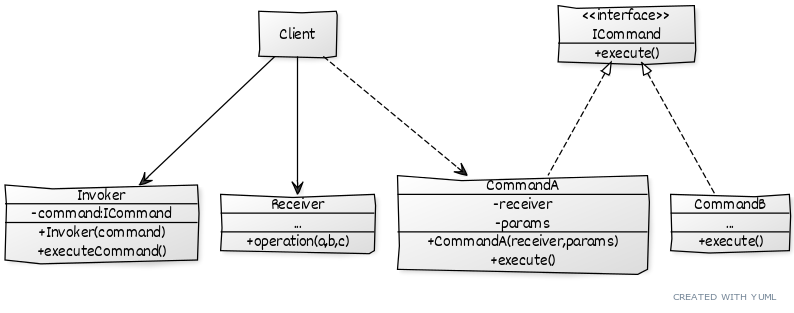
\includegraphics[width=0.9\linewidth]{images/CommandUml}
	\caption{Diagram UML wzorca Polecenie.}
	\label{lab4/fig/CommandUml}
\end{figure}
%[Client]->[Invoker]
%[Client]->[Receiver]
%[Client]-.->[CommandA]
%[ICommand]^-.-[CommandA]
%[ICommand]^-.-[CommandB]
%
%[Client]
%[Invoker|-command:ICommand|+Invoker(command);+executeCommand()]
%[≪interface≫;ICommand|+execute();]
%[CommandA|-receiver;-params|+CommandA(receiver,params);+execute()]
%[CommandB|...|+execute()]
%[Receiver|...|+operation(a,b,c)]



\subsection{Strategia (ang. strategy)}

Klient, aby zrealizować pewne zadania może wykorzystywać konkretny algorytm. Często może się on zmieniać w czasie albo być zależny od dodatkowych czynników np. wyboru opcji przez użytkownika programu. Wzorzec strategii pozwala utworzyć rodzinę realizujących dane zadanie w różny sposób algorytmów. Dalej za pomocą konstruktora, właściwości albo metody zmienić obiekt strategii i tym samym zmienić sposób realizacji danej czynności przez klienta. Gorszą alternatywą mogłoby być zbudowanie na stałe wielu algorytmów w daną klasę i naruszenie tym samym pierwszych dwóch zasad SOLID. 

Strategia bazuje na omawianej na pierwszych laboratoriach zasadzie odwracania zależności. Koncepcyjnie DI jest raczej zarezerwowane dla przypadków, gdzie podczas wykonywania się programu dane zachowanie (wstrzykiwany obiekt) jest stałe. Jeśli natomiast zakładamy, że sposób realizacji danego algorytmu się będzie zmieniał to wtedy odnosimy się raczej do strategii. Różnice między nimi są niewielkie i subtelne. Pod względem struktury strategia jest podobna również do mostu i stanu, które też bazują na kompozycji. Mimo, że pod względem struktury są ona do siebie bardzo podobne, nazewnictwo stosowane w tych wzorcach powinno dewelopera informować o specyficznym problemie, który został za jego pomocą rozwiązany.

W programowaniu obiektowym istnieje zasada, aby przekładać kompozycję nad dziedziczeniem. Podobnym do strategii wzorcem, który wykorzystuje dziedziczenie jest metoda szablonowa. Takie podejście sprawia, że strategia jest na sztywno połączona z klasa \texttt{Context}, nie możliwe jest dynamiczne zmienianie algorytmu. Dodatkowo utrudnia to zrozumienie kodu. 

%Refactoring guru
%Polecenie i Strategia mogą wydawać się podobne, ponieważ oba mogą służyć parametryzacji obiektu jakimś działaniem. Mają jednak inne cele. Za pomocą Polecenia można konwertować dowolne działanie na obiekt. Parametry działania stają się polami tego obiektu. Konwersja zaś pozwala odroczyć wykonanie działania, kolejkować je i przechowywać historię wykonanych działań, a także wysyłać polecenia zdalnym usługom, itd. Z drugiej strony, Strategia zazwyczaj opisuje różne sposoby wykonywania danej czynności, pozwalając zamieniać algorytmy w ramach jednej klasy kontekstu.



Diagram UML omawianego wzorca został przedstawiony na poniższych diagramie UML~\ref{lab4/fig/StrategyUml}. Klient tworzy obiekt konkretnej strategi (musi ona implementować wspólny dla wszystkich strategi interfejs). Dale taka instancja może zostać przekazana np. przy wykorzystaniu metody (\texttt{setStrategy(strategy)}) do obiektu realizującego daną czynność. Klient ma możliwość w trakcie działania programu płynnie zmieniać sposób realizowania danej czynności.

\begin{figure}[hbt!]
	\centering
	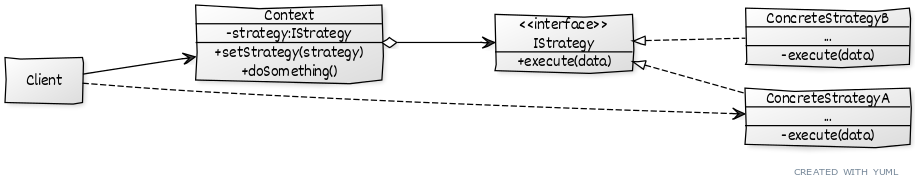
\includegraphics[width=0.9\linewidth]{images/StrategyUml}
	\caption{Diagram UML wzorca Strategia.}
	\label{lab4/fig/StrategyUml}
\end{figure}
%[Client]->[Context]
%[Client]-.->[ConcreteStrategyA]
%[Context]<>->[IStrategy]
%[IStrategy]^-.-[ConcreteStrategyA]
%[IStrategy]^-.-[ConcreteStrategyB]
%
%[Client]
%[Context|-strategy:IStrategy|+setStrategy(strategy);+doSomething()]
%[≪interface≫;IStrategy|+execute(data);]
%[ConcreteStrategyA|...|-execute(data)]
%[ConcreteStrategyB|...|-execute(data)]

Użycie wzorca strategii powinno być podyktowane faktem, że klasa korzysta z różnych algorytmów do wykonania \textbf{tej samej} czynności. Co więcej zwykle te algorytmy mogą się zmieniać w czasie. Dodatkowo algorytm ułatwia odizolowanie algorytmu od logiki biznesowej. Pozwala również ukryć szczegóły implementacyjne np. złożone struktury danych. 

Jeżeli obiekt strategi potrzebuje dodatkowych mogą one zostać udostępnione przez kontekst w momencie wywoływania algorytmu. Ewentualnie \texttt{Context} może przekazać do obiektu strategii samego siebie.

Przykładem zastosowania wzorca strategia może być nawigacja i różne algorytmy obliczania optymalnej drogi. W zależności od np. środka transportu może być stosowany inny obiekt \texttt{ConcreteStrategy}. W bibliotece \texttt{ObjectWindows} strategia jest stosowana w oknach dialogowych do sprawdzania poprawności wprowadzanych przez użytkownika danych. Zestaw oferuje część predefiniowanych algorytmów, a użytkownik jeśli nie znajdzie dla niego odpowiedniego może łatwo rozszerzyć możliwości przez stworzenie własnego obiektu implementującego konkretny interfejs. Strategia może również być wykorzystywana w algorytmach parsujących (różne algorytmy w zależności od formatu danych wejściowych) albo optymalizacji kompilowanego kodu (inne obiekty dla różnych poszczególnych rodzajów i poziomów kompilacji).

\subsection{Mediator (ang. mediator)}

Wzorzec projektowy mediator umożliwia kapsułkowanie interakcji pomiędzy obiektami poprzez dodatkowy obiekt mediatora. Obiekty mogą się komunikować jedynie przez obiekt mediatora.

%Analogią może być wieża kontrolerów lotów na lostniku. Piloci nie rozmawiają między sobą nawzajem, a komunikują się przez swego rodzaju moderatora. 

Wyobraźmy sobie sytuację, w której okno dialogowe składa się z wielu widgetów. Pewne pole może być aktywne albo nieaktywne w zależności od wybranej wcześniej opcji widgetu typu \texttt{checkbox}. W innym przypadku przycisk do wysłania formularza aktywowany jest dopiero po wypełnieniu wszystkich niezbędnych pól. Bez użycia obiektu mediatora poszczególne instancje widgetów musiałby posiadać referencje do sobie nawzajem, aby np. po zaznaczeniu pola wyboru aktywować pole tekstowe. Ponowne użycie takich elementów staje się utrudnione, a czytelność kodu pogarsza.


Zamiast zmuszać obiekty do posiadania informacji o sobie nawzajem można wprowadzić dodatkowy obiekt moderatora~\ref{lab4/fig/MediatorUml}, który będzie pośredniczył w komunikacji między obiektami. Komponenty w tej sytuacji są zależne jedynie od obiektu moderatora i to do niego kierują informację np. o zmianie stanu pola wyboru. Obiekty mogą się komunikować np. z wykorzystaniem zdarzeń albo wzorca obserwatora. Mediator jest kontrolerem we wzorcu MVC (ang. Model View Controller - Model Widok Kontroler).

\begin{figure}[hbt!]
	\centering
	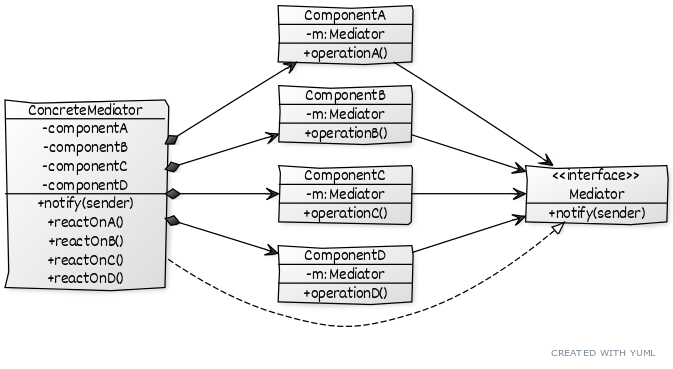
\includegraphics[width=0.9\linewidth]{images/MediatorUml}
	\caption{Diagram UML wzorca Mediator.}
	\label{lab4/fig/MediatorUml}
\end{figure}
%[ConcreteMediator]++->[ComponentA]
%[ConcreteMediator]++->[ComponentB]
%[ConcreteMediator]++->[ComponentC]
%[ConcreteMediator]++->[ComponentD]
%[Mediator]^-.-[ConcreteMediator]
%[ComponentA]->[Mediator]
%[ComponentB]->[Mediator]
%[ComponentC]->[Mediator]
%[ComponentD]->[Mediator]
%
%[≪interface≫;Mediator|+notify(sender)]
%[ConcreteMediator|-componentA;-componentB;-componentC;-componentD|+notify(sender);+reactOnA();+reactOnB();+reactOnC();+reactOnD()]
%[ComponentA|-m: Mediator|+operationA()]
%[ComponentB|-m: Mediator|+operationB()]
%[ComponentC|-m: Mediator|+operationC()]
%[ComponentD|-m: Mediator|+operationD()]

Np. w momencie kliknięcia przycisku przez użytkownika obiekt \texttt{Button} wysyła informację o operacji do mediatora, który sprawdza pozostałe pole i podejmuje decyzję np. o wysłaniu formularza. 

Wzorzec warto zastosować jeśli istnieje wiele zależności pomiędzy klasami, a ich ponowne użycie w innym programie jest z tego powodu mocno utrudnione. Podobnym wzorcem do mediatora jest fasada. Główną różnicą między nimi jest fakt, że ta druga posiada zależności jednokierunkowe. Obiekty reprezentowane przez fasadę mogą kierować żądania do podsystemów, ale podsystemy nie mogą się komunikować z fasadą.

Wadą tego wzorca jest fakt, że mediator za czasem może stać się bardzo złożony tzw. Boski Obiekt. Taki obiekt jest przykładem antywzorca projektowego. Posiada on zazwyczaj wiele zależności i łamie zasadę pojedynczej odpowiedzialności.
